\let\negmedspace\undefined
\let\negthickspace\undefined
\documentclass[journal]{IEEEtran}
\usepackage[a5paper, margin=10mm, onecolumn]{geometry}
%\usepackage{lmodern} % Ensure lmodern is loaded for pdflatex
\usepackage{tfrupee} % Include tfrupee package

\setlength{\headheight}{1cm} % Set the height of the header box
\setlength{\headsep}{0mm}     % Set the distance between the header box and the top of the text

\usepackage{gvv-book}
\usepackage{gvv}
\usepackage{cite}
\usepackage{amsmath,amssymb,amsfonts,amsthm}
\usepackage{algorithmic}
\usepackage{graphicx}
\usepackage{textcomp}
\usepackage{xcolor}
\usepackage{txfonts}
\usepackage{listings}
\usepackage{enumitem}
\usepackage{mathtools}
\usepackage{gensymb}
\usepackage{comment}
\usepackage[breaklinks=true]{hyperref}
\usepackage{tkz-euclide} 
% \usepackage{gvv}                                        
\def\inputGnumericTable{}                                 
\usepackage[latin1]{inputenc}                                
\usepackage{color}                                            
\usepackage{array}                                            
\usepackage{longtable}                                       
\usepackage{calc}                                             
\usepackage{multirow}                                         
\usepackage{hhline}                                           
\usepackage{ifthen}                                           
\usepackage{lscape}
\begin{document}

\bibliographystyle{IEEEtran}
\vspace{3cm}

\title{11.16.4.7.2}
\author{EE24BTECH11029 - J SHRETHAN REDDY}
\maketitle
% \newpage
% \bigskip
{\let\newpage\relax\maketitle}

\renewcommand{\thefigure}{\theenumi}
\renewcommand{\thetable}{\theenumi}
\setlength{\intextsep}{10pt} % Space between text and floats


\numberwithin{equation}{enumi}
\numberwithin{figure}{enumi}
\renewcommand{\thetable}{\theenumi}
\textbf{Question}:\\
$A$ and $B$ are two events such that $P\brak{A}=0.54,p\brak{B}=0.69$ and $P\brak{A \cap B}=0.35$. Find $P\brak{A^\prime \cap B^\prime}$\\
\solution\\

\textbf{Theoretical Solution:\\}
\begin{align}
	\Pr\brak{A + B} = \Pr\brak{A} + \Pr\brak{B} - \Pr\brak{AB}
\end{align}
We will start by representing $A$ and $B$ using Boolean algebra methods:
\begin{align}
	A &= AB + AB^\prime\\
	B &= AB + A^\prime B\\
	\Pr\brak{A} &= \Pr\brak{AB} + \Pr\brak{AB^\prime}\\
	\Pr\brak{B} &= \Pr\brak{AB} + \Pr\brak{A^\prime B}
\end{align}
On adding $\brak{12}$ and $\brak{13}$,
\begin{align}
	A + B &= AB + AB + AB^\prime + A^\prime B\\
	A + B &= AB + AB^\prime + A^\prime B\\
	\Pr\brak{A + B} &= \Pr\brak{AB + AB^\prime + A^\prime B}\\
	\Pr\brak{A + B} &= \Pr\brak{AB} + \Pr\brak{AB^\prime} + \Pr\brak{A^\prime B}\\
	\Pr\brak{A + B} &= \Pr\brak{AB} + \Pr\brak{A} - \Pr\brak{AB} + \Pr\brak{B} - \Pr\brak{AB}\\
	\implies \Pr\brak{A + B} &= \Pr\brak{A} + \Pr\brak{B} - \Pr\brak{AB}
\end{align}
Using the given values of $\Pr\brak{A}, \Pr\brak{B}$ and $\Pr\brak{AB}$,
\begin{align}
	\Pr\brak{A + B} &= 0.54 + 0.69 - 0.35\\
	\Pr\brak{A + B} &= 0.88\\
    \pr{A^\prime B^\prime}&=\pr{A+B}^\prime\brak{\text{demorgan's law}}\\
    \pr{A^\prime B^\prime}&=1-\pr{A+B}\\
&=1-0.88\\
    &=0.12
\end{align}
Therefore, the value of $\Pr\brak{A^\prime B^\prime}$ is $0.12$.\\\\


\pagebreak
plot for
\begin{align}
	\Pr\brak{A + B} &= \Pr\brak{A} + \Pr\brak{B} - \Pr\brak{AB}\\
    \pr{A^\prime B^\prime}&=\pr{A+B}^\prime\brak{\text{demorgan's law}}\\
    &=1-\pr{A+B}
\end{align}

\begin{figure}[h!]
   \centering
   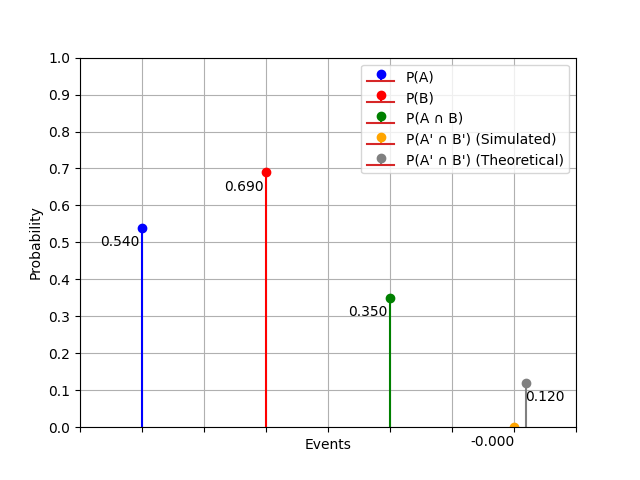
\includegraphics[width=1\columnwidth]{figure/fig.png}
   \caption{PMF}
   \label{stemplot}
\end{figure}


\end{document}
